\documentclass[journal, letterpaper]{IEEEtran}
%\documentclass{scrartcl}

\usepackage[english]{babel}
%\usepackage[latin1]{inputenc}
\usepackage[utf8]{inputenc}
\usepackage[T1]{fontenc}
\usepackage{amsmath}
\usepackage{amsthm}
\usepackage{amsfonts}
\usepackage{tikz}
\usepackage{verbatim}
\usepackage{subcaption}
\usepackage{algorithm}
\usepackage{algorithmic}
\usepackage[pdftex]{hyperref}

\renewcommand{\algorithmicrequire}{\textbf{Input:}}
\renewcommand{\algorithmiccomment}[1]{\ \ // #1} % C-like // Comments

\hyphenation{render}

% No clubs and widows allowed
\clubpenalty10000
\widowpenalty10000
\displaywidowpenalty=10000
\DeclareMathOperator*{\argmin}{arg\,min}
\begin{document}

%\title{Simulating elastic spheres without external forces}
%\subtitle{Project 1 for class CS6491 Computer Graphics}
\title{Curve Average \\
	{\large Project 3 for class CS6491 Computer Graphics}}
%\author{Sebastian Weiss}
\author{Sebastian Weiss, Can Erdogan \\ \today}
%\date{\today}

\maketitle

\begin{tikzpicture}[remember picture,overlay]
   \node[anchor=north east,inner sep=0pt] at (current page.north east)
              {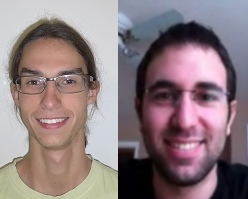
\includegraphics[scale=1.5]{pic}};
\end{tikzpicture}

\section{Objective}
Formally, for two curves $A = \{a_0 ... a_{n-1}\}$ and $B = \{b_0 ... b_{n-1}\}$, each with $n$ points and $\forall x \in (A \cup B), x \in \mathcal{R}^3$,
the goal is to find a curve $C$ such that for each point $c \in C$, and its closest projections
\begin{align}
a^c &= \operatornamewithlimits{argmin}\limits_{a \in A} ||a-c|| \text{, and} \\
b^c &= \operatornamewithlimits{argmin}\limits_{b \in B} ||b-c||
\end{align}

\noindent the following holds true:

\begin{equation}
 c = \operatornamewithlimits{argmin}\limits_{x \in L(a^c, b^c)} ||a^c-x||
\end{equation}

\noindent where for each point $r$ on line $L(p,q)$, $||r-p|| = ||r-q||$. Moreover, for
any three consecutive sampled points $c_i$, $c_j$ and $c_k$ on curve $C$, the arc lengths
of the curves between their closest projections are the same:
\begin{equation}
\small
 D^A(a^{c_i},a^{c_j}) + D^B(b^{c_i},b^{c_j}) = D^A(a^{c_j},a^{c_k}) + D^B(b^{c_j},b^{c_k})
\end{equation}
\noindent where $D^Z(x,y)$ is the distance along the curve $Z$ between points $x,y \in Z$.

Semantically, we want to find the curve that is composed of the loci of the smallest spheres that touch the two inputs curves A and B,
and sample it such that for each sample on the curve, the distances traveled by the matching samples along their curves is a constant.

\section{Input}
The input is the six control points for two curves $A$ and $B$, named $A_0$ to $A_5$ and $B_0$ to $B_5$, such that the first and the last control points are the same.

\section{Overview}
The project is composed of the following three main parts: (1) the representation of the curves,
(2) the computation of the average curve, and (3) the visualization of the different curve properties.
The challenge in the representation is that we want the spline curves to first meet at two end points and then,
to have $C^1$ continuity at the intersection of the splines. For the curve average, we had to ensure
the points satisfied the constraints in Equations 1-3. Lastly, the visualization contained multiple challenges
including parallel transport, circular arc computation and etc.

\section{Curve Representation}
We compose each curve out of piecewise quadratic Hermite and cubic Hermite splines. Each spline is connected at a control point by the same local velocity. This leads to a $\mathcal{C}^1$-smooth curve.
We define the tangent/velocity at control point $A_i$ as $T_i = c*(A_{i+1}-A_{i-1})$. The parameter $c$ defines the curvature or the influence of that velocity. In our experiments, we set $c$ to 0.5.

A cubic Hermite spline requires velocities at both end points, a quadratic Hermite spline only at one end point. Therefore, we use the quadratic form for the first and the last part of the curve and the cubic form for all middle parts.

\subsection{Quadratic Hermite Spline}
Given the points $X_0$ and $X_1$ and the tangent $T_0$, find a quadratic spline $P(t)$ so that the following holds:
\begin{equation}
\small
 P(0)=X_0, P(1)=X_1, P'(0)=T_0
\end{equation}
Solving this system of equation leads to the following formula:
\begin{equation}
\small
 P(t) = (t^2-2t+1)X_0 + (-t^2+2t)X_1 + (t^2-t)T_0
\label{eq:QuadraticHermite}
\end{equation}

\subsection{Cubic Hermite Spline}
Given the points $X_0$ and $X_1$ and the tangents $T_0$ and $T_1$, find a cubic spline $P(t)$ so that the following holds:
\begin{equation}
\small
 P(0)=X_0, P(1)=X_1, P'(0)=T_0, P'(1)=T_0
\end{equation}
This equation is solved similar to the quadratic case, leading to:
\begin{equation}
\small
 P(t) = (2t^3-3t^2+1)X_0 + (t^3-2t^2+t)T_0 + (-2t^3+3t^2)X_1 + (t^3-t^2)T_1
\label{eq:CubicHermite}
\end{equation}

\section{Average Curve Computation}

\subsection{Distance functions}
\subsection{Average Distance Sampling}

\section{Visualization and Editing}

\begin{figure*} %This just must appear at the page before the chapter "Displaying the average curve"
	\centering
		\begin{tabular}{cccc}
			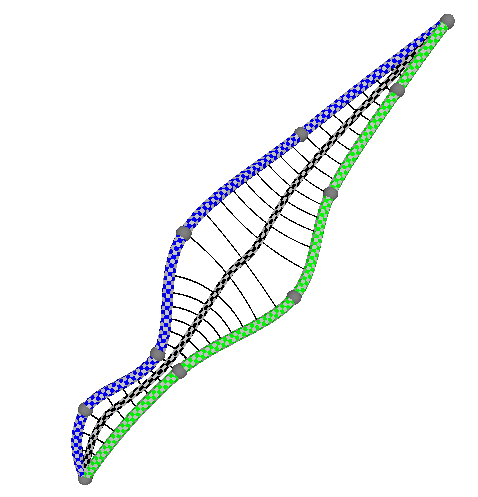
\includegraphics[scale=0.5]{images/NoGeodesicSampling.png} & 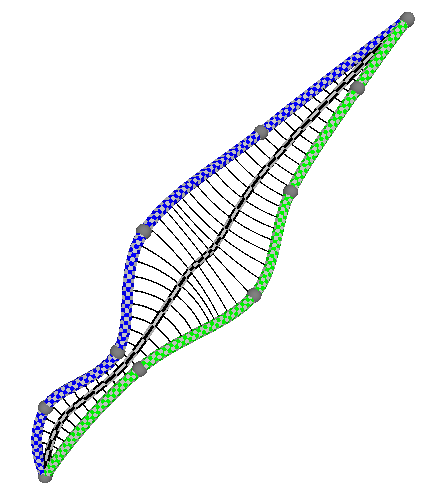
\includegraphics[scale=0.5]{images/GeodesicSampling.png} 
				& 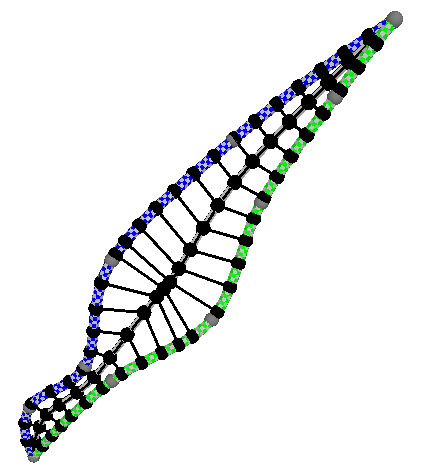
\includegraphics[scale=0.5]{images/ClosestProjections.png} & 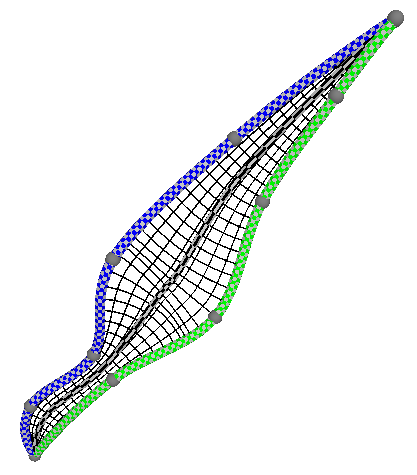
\includegraphics[scale=0.5]{images/CircularArcNet.png} \\
			a) no geodesic sampling & b) with geodesic sampling & c) the closest projections & d) net of circular arcs
		\end{tabular}
	\caption{Geodesic sampling, closest projections and circular arcs}
	\label{fig:GeodesicSampling}
\end{figure*}

We provide a framework for editing the control curve and visualizing the curve average.
More specific, we support the following features: 
\begin{itemize}
	\item Moving the control points of the two input curve
	\item Displaying the curve average with or without geodesic sampling
	\item Displaying the closest projections
	\item Displaying the circular arc and animating the curve average along it
	\item Showing the inflation tube, the envelope of the smallest spheres
\end{itemize}
We now describe the single features in more detail

\subsection{Editing and displaying the control curve}
We display the control points as gray spheres and the two control curves in green and blue.
The user can click the control points and change their positions by dragging them over the screen.

\subsection{Displaying the average curve}
The curve average is displayed by connecting the sample points using piecewise straight tubes. The faces of the tubes are rendered in alternating black and gray so you can see where the trace points are.
The user has now the option to toggle geodesic sampling on or off. The effects are shown in Fig.\ref{fig:GeodesicSampling}ab. 

As you can see, without geodesic sampling, the distances between the samples of the curve average are almost equispaced, but the closest projections on the control curve, indicated by the circular arcs, vary greatly in the distances. With geodesic sampling turned on, the curve average is sampled in that way that the sum of the distances between two consecutive closest projects on the control curves are constant. However, this leads to large variation of the distances of the curve average samples.

\subsection{ClosestProjections}
To visualize the closest projections, i.e. the points on the control curve that are closest to the average curve at this point, we draw straight lines between the sample of the curve average and its closest projections. These can be seen in Fig.\ref{fig:GeodesicSampling}c. Note that the lines to both control curves are of the same length and that they stand orthogonal to the control curve at the intersections. These are the properties that define the closest projections and the curve average.



\section{Results}

\section{Future work}

\end{document}